\section{Environment plugin development (WP5)}

The articles mentioned in part \ref{WP3} describe quite precisely the algorithms usable to build and merge the different features. The work done for the code of the environment part was to organise the different algorithms into several classes (summarised on Figure \ref{env_classes}). The main classes are:

\begin{description}
  \item[Feature] This class is like an abstract class. It is the base from which every feature inherit, to allow us to manipulate generic feature in our code.
    \item[FeatureTree] This class build the tree of the features, depending on their positions and thus their interactions. It also solves the ``merge'' of the different features.
    \item[Environment] This one is the final 3D environment, which uses the 3D models and the feature tree to build the 3D environment.
    \item[BlendEnvironment] This class is the only one depending on Blender, it converts the Environment class to allow it to be displayed and used into Blender.
\end{description}

\begin{figure}[h]
  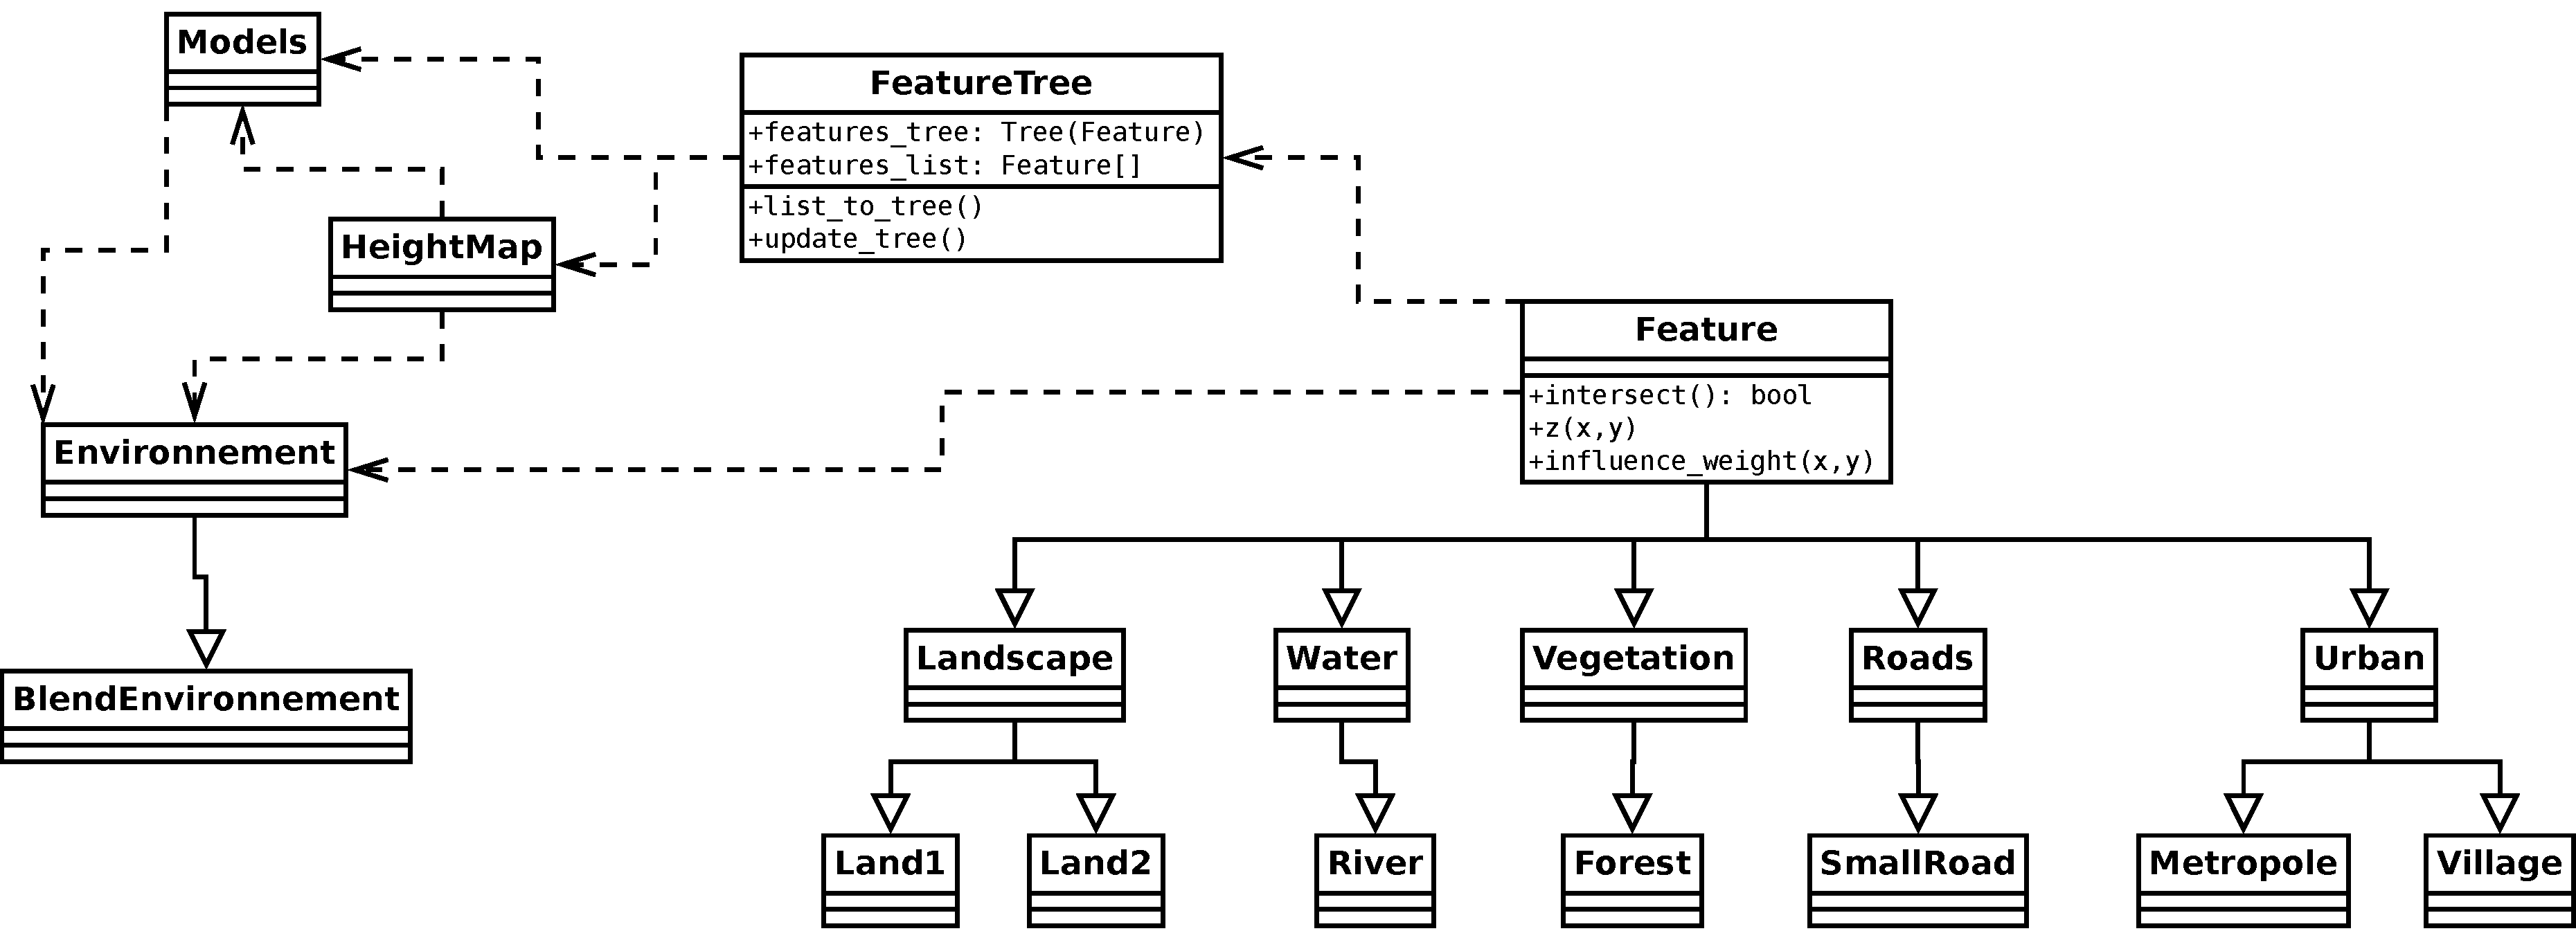
\includegraphics[width=15cm]{env_final.pdf}
  \caption{Classes of \texttt{environment plug-in} and relations between them.}
  \label{env_classes}
\end{figure}
